\documentclass{scrartcl}
\usepackage{dominatrix}
\begin{document}
  \begin{framed}
  \large
  CS 5220 Applications of Parallel Programming \hfill Fall 2015 \\
  Kenneth Lim (\href{mailto:kl545@cornell.edu}{kl545}) \hfill Intro. to Parallel Machines and Models \hspace{-3ex}
  \end{framed}
  \begin{enumerate}
    \item
    \begin{figure*}[ht!]
      \centering
      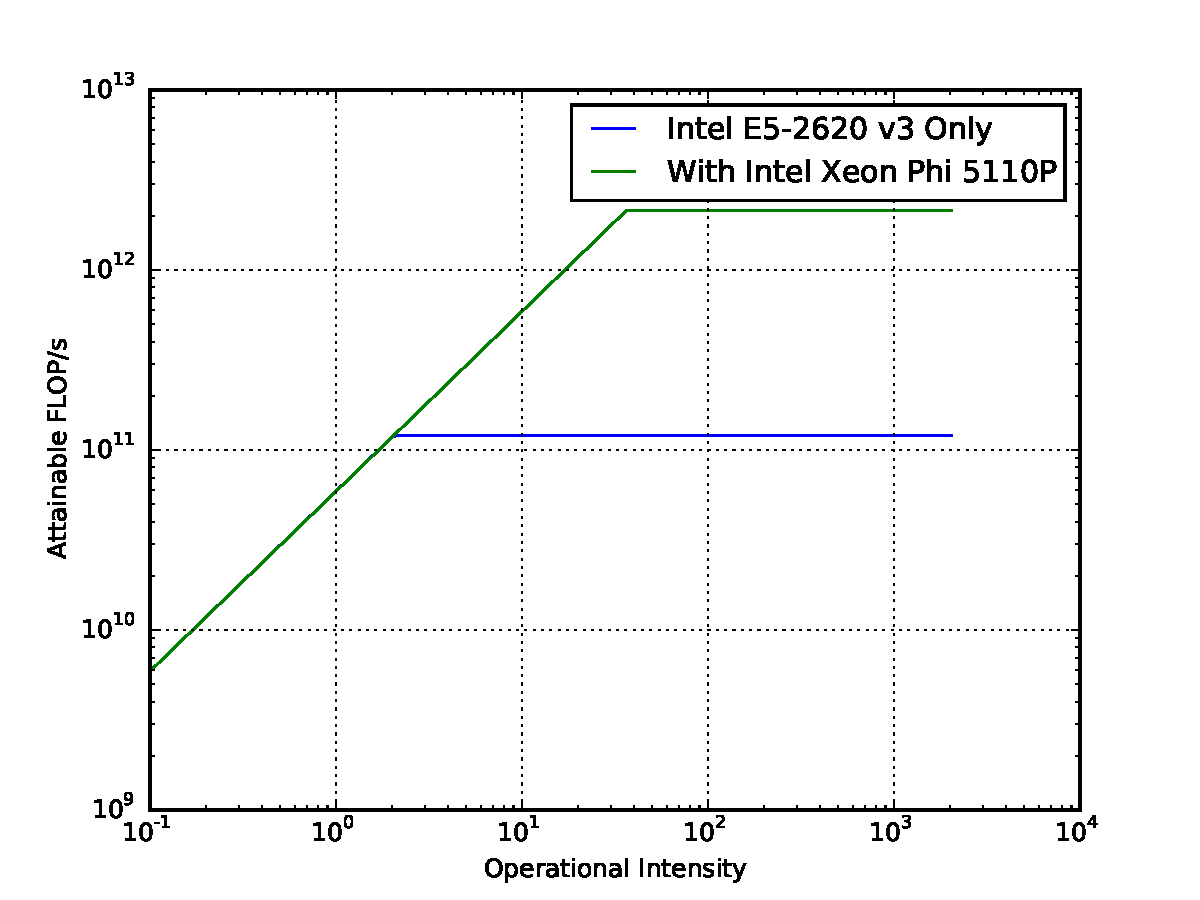
\includegraphics[width=0.75\textwidth]{roofline}
    \end{figure*}
    The peak memory bandwidth of a single totient node is 59 GB/s, and the peak flops is 120 GFlops/s. Thus the roofline diagram increases monotonically till an inflection point at (120/59, 120), after which it plateaus. The addition of the two Phi boards will increase the peak flop rate, but not change the memory bandwidth because the processor is the bottleneck.
    \item A physical core with hyperthreading can simulate the presence of two logical cores with independent execution of two different processes. However, both logical cores still share the same execution resources, whereas a setup with two physical cores has two separate sets of execution resources.
    \item For this bit, we'll consider the Knights' Landing version of the Intel Xeon Phi architecture. Memory is accessed via a bidirectional ring interconnect with memory controllers symmetrically interleaved around the ring (between cores). There is an all-to-all mapping from tag directories to memory controllers, and addresses are uniformly distributed. Memory access is non-uniform.
    \item Let the number of processors be $p$, the communication overhead per processor be $c$, the time taken to perform a floating point operation be $f$, and the size of the vectors be $n$. Then a dot product operation takes $(2n)f$ time in serial execution. In parallel execution, we incur $cp$ communication overhead, but can distribute the $2nf$ serial time over $p$ processors. Thus the speedup is:
    \[
      \frac{2nf}{\frac{2nf}{p} + cp} = \frac{2nfp}{2nf + cp^2}
    \]
  \end{enumerate}
\end{document}
